\chapter{Introduction}

%%The merger of two white dwarfs (WDs) originally in a short-period binary is estimated (eg. \citealt{badem12}) to occur about once every century in a Milky Way-like galaxy, making the products of such events common throughout the universe.  They have been held responsible for producing a variety of stars with strange properties, including helium-burning sdOB stars \citep{saioj00, justph11}, RCrB stars (eg. \citealt{webb84, clay+07, clay13}), and massive and highly magnetized WDs (eg. \citealt{segrcm97, garc+12, kule+13}) that could resemble the hot DQ WDs (eg. \citealt{dunlc15}, Dunlap and Clements in preparation).  They may, however, also be responsible for spectacular transient events including accretion-induced collapses (eg. \citealt{saion85, abdi+10}) and type Ia supernovae (SNe Ia; eg. \citealt{howe11, hill+13, maozmn14}).  Determining the final outcome of a particular merger requires an understanding of the detailed dynamics of the merging process, which cannot directly be seen using current observational capabilities.  Thus, studies of merger physics have primarily utilized hydrodynamic simulations.

Approximately two out of every three stars are born into a binary system.  A substantial fraction of these stars will interact, some following the expansion of one or both constituent stars as they evolve off of the main sequence, and others after gravitational radiation, magnetic braking or three-body dynamics drastically shrink their orbital separation.  These interactions primarily take the form of mass transfer between the stars, and if mass transfer becomes unstable, it ends with the violent coalescence of the two stars into one.  These stellar mergers, like other forms of binary interaction, disrupt single star evolution and create merged products, or ``merger remnants'', with unusual properties.

%eg. V838 Monocerotis and V1309 Scorpii 

Mergers also liberate energy on the order of the gravitational binding energy of the binary and can eject copious amounts of mass, giving rise to a cornucopia of electromagnetic (and gravitational-wave) transients ranging from luminous red novae (from the merger of two (post-) main-sequence stars; eg. \citealt{tyle+11, nandil14}) to short gamma-ray bursts (from two neutron stars or a neutron star and a black hole; eg. \citealt{ross15}) and the gravitational wave outburst from coalescing stellar-mass black holes (as recently found by the Advanced Laser Interferometer Gravitational-Wave Observatory (Advanced LIGO); \citealt{ligo16}).  Indeed, with current deep and short-cadence optical/near-infrared survey projects such as the Palomar Transient Factory \citep{rau+09} and Pan-STARRS \citep{kais+10} continuing to uncover more uncommon and even hitherto-unknown transients, and the ambitious Large Synoptic Survey Telescope \citep{lsst09} under construction, a much more complete picture of merger-generated transients will form over the next decade.

In this thesis, I will be examining the merger and post-merger evolution of two carbon-oxygen white dwarfs to determine the sorts of merged products and transients they create.  In particular, I investigate if they can produce thermonuclear, or Type Ia, supernovae, even if their total mass is below the Chandrasekhar mass.  I will first discuss the mergers of white dwarfs in general, and the diverse array of unusual stars and explosions they could potentially generate.  I will then focus on the possible outcomes for mergers of sub-Chandrasekhar carbon-oxygen white dwarf binaries, and elaborate on why novel mechanisms for making Type Ia supernovae are needed.

% Sec 5.2.3 of Tylenda talks about MS - MS pre-merger orbital evolution.

\section{Mergers of Two White Dwarfs}
\label{sec:c1_wdmergers}

Stars with masses $\lesssim8\,\Msun$ generally end their lives as white dwarfs (WDs).  On their own, WDs are inert: held up against gravity by electron degeneracy pressure and having ceased nuclear fusion, they will slowly radiate away their remaining thermal energy over billions of years.  WDs in interacting binaries, on the other hand, can receive mass and energy from their stellar companion, leading to a whole host of energetic and potentially explosive phenomena.

%\subsection{The Formation of Double White Dwarf Binaries}
%\label{ssec:c1_ddwdform}

Among double WD binaries, a fair number are in extremely close orbits, with periods ranging from hours to minutes.  As these periods correspond to orbital separations well within the radii of red and asymptotic giant branch stars, the WD pairs are formed from systems that have experienced at least two episodes of mass transfer (eg. \citealt{nele+01a, toonnp12, toon+14}).  These can sap the orbital angular momentum of the binary through mass loss, and so close double WDs tend to come from systems where (at least) the final mass transfer phase is a ``common envelope event'' where one star enters the envelope of the other and much of this envelope is ejected.\footnote{Binaries may also experience a ``double common envelope event'' -- where both stars simultaneously envelop one another -- and other unusual interactions.  See eg. \cite{toonnp12} and the Appendix of \cite{toon+14} for overviews of the formation channels of close double WD binaries.}

%http://adsabs.harvard.edu/abs/2008MNRAS.387.1693C
%The mass parameter space of double WD binaries, subdivided by their chemical composition,
\begin{figure}
\centering
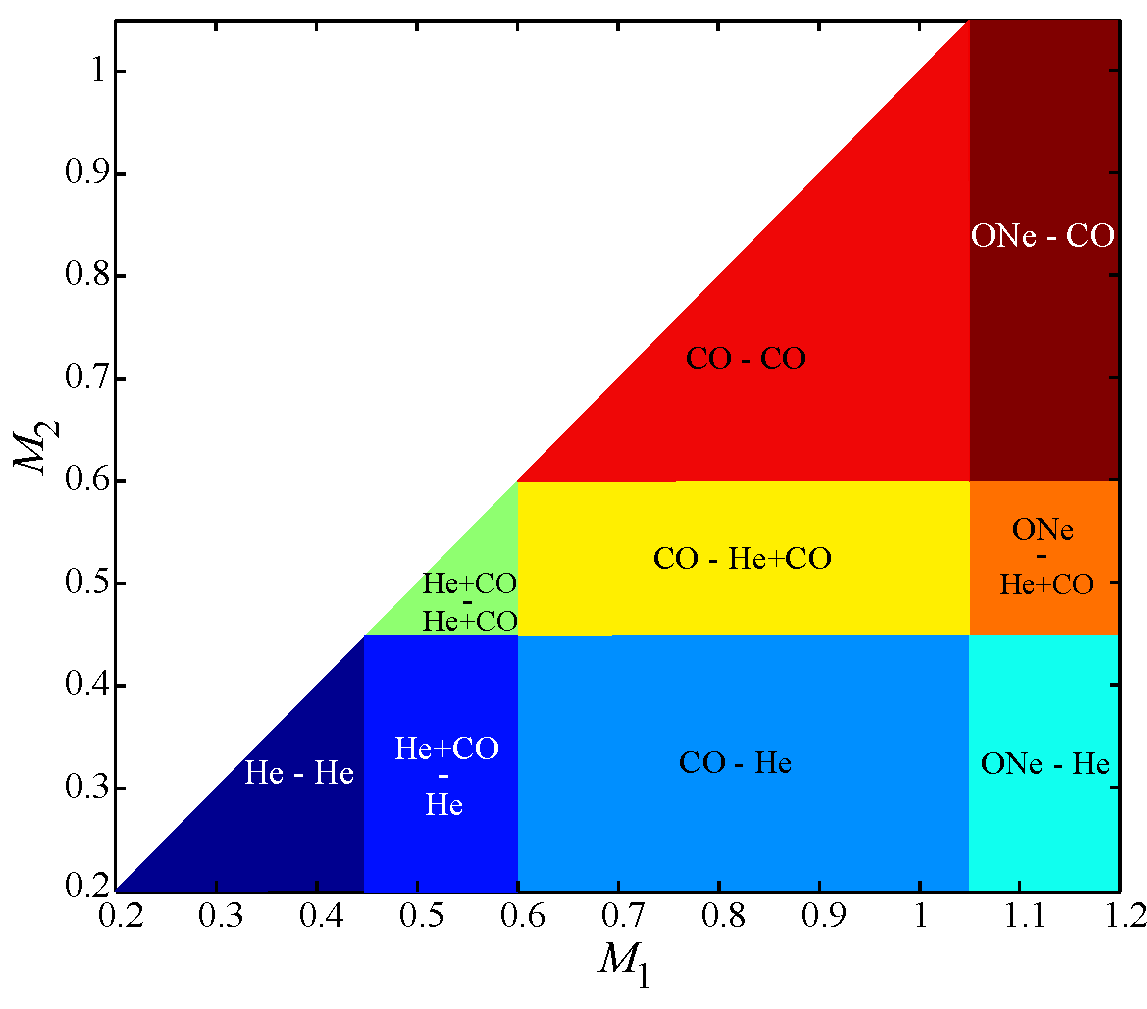
\includegraphics[width=0.6\hsize]{introduction/figures/dan+12_wdbinmass.pdf}
\caption{The expected compositions for white dwarfs undergoing a merger as a function of their masses, from \citeauthor{dan+12} (\citeyear{dan+12}, their Fig. 1).  $M_1$ is the mass of the accretor, or primary, WD (\Ma\ in the text), and $M_2$ is the mass of the donor, or secondary (\Md).  WDs with masses $M<0.45\,\Msun$ are assumed to be He WDs, those with $0.45 < M < 0.6\,\Msun$ CO WDs with thick He envelopes, $0.6 < M < 1.05\,\Msun$ CO WDs, and $M>1.05\,\Msun$ ONe WDs.  See text, as well as \cite{dan+12} Sec. 2, for discussion on these choices.}
\label{fig:c1_wdbinarymasses}
\end{figure}

% He flash - eg. \citealt{kippww12}, Ch. 33.4
% He WDs need friends: eg. \citealt{kippww12}, Ch. 33.4
% Overview of He WD origins (http://adsabs.harvard.edu/abs/2012A&A...547A..96C)

The mass and composition of each WD within the binary is dependent on the binary's prior evolution.  Broadly speaking, WDs with masses $M \lesssim 0.45\,\Msun$ are composed of helium (He); these come from stars that had their evolution interrupted by binary interaction while on the red giant branch {\charles (eg. \citealt{mars95, nele+01a, podsrp02, nelsdm04}), before their degenerate He core became massive enough to trigger a helium flash.\footnote{{\charles WDs with $M\lesssim0.5\,\Msun$ could also come from single stellar evolution, but, except in cases of extreme mass loss on the red giant branch (eg. \citealt{kali+07}), this would take longer than a Hubble time.}}  WDs with slightly higher masses have cores composed of carbon and oxygen (CO) surrounded by extensive He envelopes of $\sim0.1\,\Msun$ (eg. \citealt{ibent85, nele+01a, podsrp02}).  \cite{dan+12}, who simulate mergers of WDs with masses from $0.2 - 1.2\,\Msun$, approximate the mass range of these ``hybrid WDs'' to be $0.45 \lesssim M \lesssim 0.6\,\Msun$, and set the composition of the upper $0.1\,\Msun$ of their WDs that are within this range to He.}  From $0.6 \lesssim M \lesssim 1.1\,\Msun$ WDs are almost entirely composed of CO, with He atmospheres of $\sim10^{-2}\,\Msun$ \citep{ibent85}.  WDs with masses $\gtrsim 1.1\,\Msun$ come from super-AGB stars (eg. \citealt{herw05, garc13}) that ignite carbon during their evolution, and thus are composed at least partly of oxygen and neon (ONe).  

Fig. \ref{fig:c1_wdbinarymasses}, from \cite{dan+12}, summarizes these relationships -- in it, $M_1$ is the mass of the more massive primary WD, which accretes mass during the merger, and $M_2$ is the mass of the secondary, which donates mass (see Sec. \ref{ssec:c1_stable_mass_transfer} for why this is always the case).  In this thesis, we refer to these as \Ma\ and \Md, respectively.  While sophisticated stellar evolution calculations are {\charles not at all as} clear-cut (eg. \citealt{ibent85, moros09} for CO WDs with $M\lesssim0.45\,\Msun$ and \citealt{hurlpt00} for CO WDs with $M\gtrsim1.2\,\Msun$), these relationships are used as rules of thumb for setting WD composition for a wide range of works (\citealt{loreig09}, henceforth \citeal{loreig09}; \citealt{rask+12,dan+12,dan+14}), with slight variations between them.  In this thesis, we look at binaries of pure CO WDs (without He atmospheres) with masses ranging from $0.4 - 1.0\,\Msun$.

% for our parameter space study of mergers in Ch. \ref{ch:ch2}.  

%In subsequent chapters, we are primarily interested in the the merger of two CO WDs near the median mass of field WDs, $\sim0.65\,\Msun$ (Sec. \ref{ssec:c1_cowd_massrange}).

%The ratio of carbon and oxygen within CO WDs is also not particularly well-known.  In this thesis, we make the assumption that they are composed of 50\% carbon and 50\% oxygen by mass.  {\charles ADD STUFF}

%\subsection{Orbital Angular Momentum Loss and Gravitational Wave Emission}
%\label{ssec:c1_inspiral}

%magnetic braking ({\charles important for AM Canum Venaticorum systems} eg. \citealt{verb84, knigbp11})

Following their formation, WD binaries lose orbital angular momentum by emitting gravitational radiation (eg. \citealt{petem63}).\footnote{They may also lose angular momentum through the influence of a third body (eg. \citealt{katzd12}); see Sec. \ref{ssec:c1_new_typeia}.}  This loss has a characteristic inspiral timescale of \citep{segrcm97}

\begin{eqnarray}
\tau_{\mrm{grav}} = \frac{L_\mrm{orb}}{|\dot{L}_\mrm{orb}|} &=& \frac{5c^5}{32G^3}\frac{a^4}{\Ma\Md\Mtot}\nonumber \\
&=&5 \times 10^5 \left(\frac{a}{10^5 \mrm{km}}\right)^4 \left(\frac{\Msun}{\Ma}\right) \left(\frac{\Msun}{\Md}\right) \left(\frac{\Msun}{\Mtot}\right)\,\mrm{yr}.
\label{eq:c1_gravtimescale}
\end{eqnarray}

\noindent where $L_\mrm{orb}$ is the orbital angular momentum and $a$ is the orbital separation.  From this, we see that WD binaries with orbital periods on the order of hours or less ($a \lesssim 10^6\,\mrm{km} \sim 0.01\,\mrm{AU}$) will merge within a Hubble time.  

%It is estimated that there are on order of $10^8$ such systems in the Milky Way alone \citep{mars11, nele+01a}. <- This may be somewhat true, but don't write this unless you can guarantee all of these will merge within a hubble time!

As an aside, the gravitational waves emitted by inspiralling WD binaries are detectable from Earth.  With periods on the order of minutes, they are too low-frequency to be detected by Advanced LIGO \citep{ligo+15}, but are expected to be the most numerous and dominant source of gravitational waves \citep{mars11} detected by the proposed spaceborne detector eLISA (evolved Laser Interferometer Space Antenna; \citealt{amar+13}), which probes the mHz - Hz frequency range.  The instrument will likely resolve individual signals from thousands of binaries with orbital periods on the order $\sim10$ minutes (and are thus close to merging; \citealt{amar+13, mars11, dan+11}), while numerous sources that are too far away or at longer orbital periods will comprised an unresolved background \citep{neleyp01,amar+13}.  Measurement of either of these will probe the WD binary population of the Milky Way without the selection biases that often trouble electromagnetic binary searches \citep{mars11}.  Note that gravitational radiation plays a negligible role in the actual merger, as the waves released during the merger have a total energy $\sim10^{-10}$ of the binary's binding energy (eg. \citeal{loreig09}).

%Note, however, that final coalescence of the WDs is over far too quickly to be detectable by eLISA.

\section{Merger Outcomes}
\label{sec:c1_mergeroutcomes}

Like any merger, those between WDs liberate of order their gravitational binding energy.  This can lead to enough heating and/or compression to reignite the nuclear furnaces of normally inert WDs.  As this may happen under either non-degenerate or degenerate circumstances, the end product of such mergers are diverse, ranging from stars with unusual properties undergoing stable nuclear burning to explosions. Additionally, hydrostatic WDs have a maximum mass beyond which they are unstable to collapse -- the \cite{chan31} mass, or \Mch, at $\sim1.4\,\Msun$.  This has long led to the notion that sufficiently massive WD mergers can result in the complete destruction of the merger product in a thermonuclear explosion that would resemble a Type Ia supernova (SN Ia; \citealt{webb84}), or in its transformation into a neutron star (NS; \citealt{nomoi85, saion85}).  We now know of a much greater range of possible merger outcomes for both systems with masses above and below \Mch.  Which outcome occurs depends on the compositions of the WDs involved, and are briefly summarized below (see also \citealt{dan+14}, who produce a similar list):

% dan+14 Fig 12, dan+12 fig 8

\begin{itemize}
	\item The merger of {\bf two He WDs} is unlikely to lead to violent nuclear burning and an explosion \citep{dan+12,dan+14,dan+15}.  Instead, merger remnants with total masses $0.4\lesssim \Mtot \lesssim 0.8$ \citep{han+02,ibent85}\footnote{This is lower than the He flash mass of $\sim0.45\,\Msun$ because the merger remnant is partly non-degenerate \citep{ibent85, han+02}.}, which are the vast majority of double He WD remnants \citep{nele10}, are expected to ignite He burning in a shell.  \cite{saioj00} and \cite{zhanj12} calculate that He shell burning increases the radius and luminosity of the remnant, turning it over $\sim 10^3-10^4\,\mrm{yr}$ into a yellow giant.  Over the next $10^5-10^6\mrm{yr}$, the burning shell migrates inward with a series of weakening shell flashes, while the radius slowly shrinks to $\sim10^{-1}\,\Rsun$.  Once the shell reaches the center of the remnant, the remnant settles onto the helium main sequence, and resembles a He-rich subdwarf B (sdB) or O (sdO) star \citep{saioj00, justph11, zhanj12, hebe16}.  Most subdwarf stars are in binaries -- and likely arise from other formation channels -- and there are multiple mechanisms theorized to produce single sdB stars (such as a merger between a low-mass star or brown dwarf and a red giant; \citealt{soke98}), and so the contribution of mergers to the sdB population remains unclear \citep{nele10, hebe16}.

%"with properties similar to Extreme Helium (EHe) and R Coronae Borealis (R CrB) stars \citep{saioj00, zhanj12}", but this then makes the description too confusing.

% See conclusion section of hebe16 for alternate sources of single subdwarfs.  From hebe16: single sdBs tend to be narrowly peaked in mass, not obvious if mergers can do this.  Low mass MS star or brown dwarf may merge with RGB core to make single sdB in CE, He WD/MS merger.  From nele10: enhanced single star mass loss might do it too, but not obvious if this happens

%(\citealt{justph11}; He-poor sdO stars are likely evolved sdB stars)

	\item The outcome of a merger between {\bf an He and a CO WD}, or a merger between an He and hybrid He-CO WD, depends on whether or not an He explosion is touched off during the merger.  Roughly speaking, mergers with $\Mtot \lesssim 0.8\,\Msun$ will lead to steady He burning in a shell, and are thought to be the progenitors to He-rich sdO stars \citep{justph11}.  Mergers with $\Mtot \gtrsim 0.8\,\Msun$ that do not experience an explosion will also ignite shell burning, but unlike their less massive counterparts they will retain their extended envelope over the $\sim10^5\,\mrm{yr}$ lifetime of the He-burning shell \citep{ibent85, zhanj12b}.  These mergers are believed to be the primary formation channel for Hydrogen-deficient Carbon (HdC) and R Coronae Borealis (R CrB) stars (eg. \citealt{webb84, ibent84, saioj02, clay12, zhan+14}), which are H-deficient, He- and C-rich supergiants that, in the case of R CrB stars, feature abrupt variability by up to a factor of $\sim10^3$ due to the formation of carbon dust above their photospheres.\footnote{Subdwarf stars formed from double He WD mergers with $\Mtot \gtrsim 0.8\,\Msun$ will also expand to become R CrB stars following core He exhaustion, but this formation channel accounts for only a few percent of all R CrBs \citep{zhanj12b}.}  Following He shell exhaustion, they will contract in radius and heat their envelopes, resembling EHe stars \citep{saioj02, jeff14} before eventually becoming CO WDs.

Helium explosions become more likely for binaries with $\Mtot\gtrsim\Mch$ \citep{dan+12, dan+14}.  In cases where an accreted He shell explodes, but the underlying CO WD remains, the result depends on a number of factors including the mass of the CO WD and amount of He it accretes, and spans a wide range of possible peak luminosities \citep{shen+10he, wald+11, woosk11}.  Detonations (or deflagrations; \citealt{woosk11}) of $\lesssim0.1\,\Msun$ He shells lead to explosions that reach peak brightnesses $\sim10-100$ fainter than SNe Ia over $\sim2-10$ days (typical SNe Ia values are in Sec. \ref{sec:c1_mysteryofsneia}), making them similar to the ``.Ia SNe'' theorized to occur in AM Canum Venaticorum binaries \citep{bild+07}.  They synthesize Ca, Cr and Ti, but relatively little of the radioactive \Ni\ typically seen in SNe Ia \citep{shen+10he, woosk11, wald+11}.  Denser He envelopes (which are either themselves more massive or lie over more massive CO cores), tend to synthesize more \Ni\ in detonations \citep{shen+10he, wald+11}. 

%As an aside, \cite{wald+11} also suggest that the detonation of $\sim0.2\,\Msun$ of He on top of a $\sim0.45\,\Msun$ CO WD could explain the SN 2005E-like class of low-luminosity SNe Ib that produce very little \Ni, have low ejecta masses and spectroscopically show strong lines of He, Ca and Ti \citep{pere+10}.  Their initial conditions (and those of \cite{shen+10he}) assume the He envelopes were constructed through slow ($\lesssim10^{-6}\,\Msun\,\pyr$) accretion onto the CO cores until He nuclear runaway is triggered through compressional heating.  Mergers between low-mass CO and He WDs will likely generate He envelopes that are far less degenerate, and which will not experience such a nuclear runaway.

% moreover simulations suggest He detonations in mergers occur before an He envelope of more than a few $10^{-2}\,\Msun$ can accrete onto the disk.

%Less degenerate material will lead to explosions dominated by lighter elements like Ca \citep{woosk11}, and therefore He detonation may be possible in really massive systems.  Dan+14 already had that idea though; see below.

In the case where the He shell detonates, and triggers the CO WD to do the same, a ``double-detonation'' SN Ia may be produced (Sec. \ref{ssec:c1_new_typeia}).

	\item The merger of {\bf two CO WDs} has long been suspected of producing an SN Ia under the right conditions (Sec. \ref{sec:c1_mysteryofsneia} and \ref{sec:c1_vkchannel}).  If these conditions are not met, they will instead create a lone, massive, rotating and highly magnetized CO WD or, if steady carbon fusion is ignited, a carbon-burning star that eventually turns into an ONe WD (Sec. \ref{sec:c1_hotdqs}).  If the ONe WD is above \Mch, it may collapse into a neutron star (see below).

	\item Due to their mass, it is likely that the merger of {\bf an ONe WD} with any companion will create a super-\Mch\ remnant.  Unlike their CO counterparts, an ONe WD that is compressed through accretion to $\gtrsim3\times10^9\,\gcc$ initiates electron-capture reactions onto $^{20}$Ne and $^{24}$Mg, losing degeneracy support in the process (eg. \citealt{miya+80, saion85, schwqb15}).  This leads to further contraction, which likely ends\footnote{Since the electron capture reactions are exothermic, they trigger a thermal runaway that eventually starts an O-deflagration at $\sim10^{10}\,\gcc$.  Whether or not collapse or explosion occurs depends on exactly when the deflagration ignites; see eg. discussion in \cite{schwqb15}.} in an accretion-induced collapse (AIC) into a neutron star soon after its central density reaches $\sim10^{10}\,\gcc$ \citep{schwqb15}.  Simulations \citep{dess+06, dess+07, frye+09} of the AIC find it expels only $\sim10^{-2}\,\Msun$ of ejecta and produces negligible amounts of radioactive \Ni, suggesting a very faint transient.

%Note - oxygen pycnonuclear fusion occurs well beyond 10^10 gcc (Fig. 12 Schw+15)

\cite{dan+14} discusses the possibility that He - ONe and CO - ONe WD mergers will lead to enshrouded AIC that produce ``hybrid supernovae'', where much of the outer envelope (of a different composition) explodes rather than collapsing.  In particular, they suggest (based on the \cite{shen+10he} and \cite{wald+11} simulations above) that the detonation of the thick He envelope of a significantly super-\Mch\ He - ONe WD merger remnant could  explain the SN 2005E-like class of low-luminosity SNe Ib that produce very little \Ni, have low ejecta masses and spectroscopically show strong lines of He and Ca \citep{pere+10}.

\cite{marq+15} suggest that an ONe WD could be detonated through binary interactions in the same manner as CO WDs (Sec. \ref{ssec:c1_new_typeia}).  Due to their high densities, these would produce $\gtrsim1\,\Msun$ of \Ni, but, because fusing to \Ni\ from O and Ne generates $\sim30$\% less energy than from C \citep{marq+15}, they would also be weaker than CO WD detonations.  Detonations during ONe mergers may explain supernovae such as SN 2009dc \citep{taub+09} that have a peak brightness $\sim3$ times higher, and decay from peak brightness $\sim3$ times more slowly, than SNe Ia, and also have low expansion velocities.

\end{itemize}

Of these possibilities, ones that create SNe Ia are particularly intriguing, as they may hold the key to solving the long-standing problem of how these explosions arise.
